% Канонический TikZ-рисунок варианта 20. Править только здесь.
\long\def\figStereoV20{%
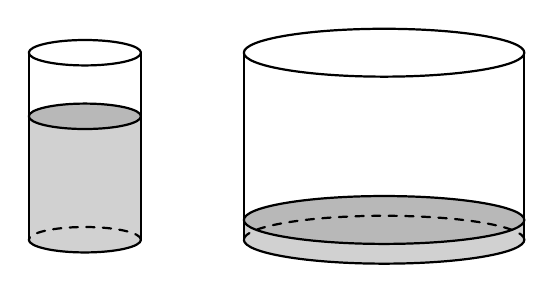
\begin{tikzpicture}[
  scale=0.95,
  line cap=round,
  line join=round
]
  % Первый сосуд
  \def\rone{0.75}
  \def\hone{2.5}
  \def\waterone{1.65}

  % Жидкость
  \fill[black!18]
    (-\rone,0) rectangle (\rone,\waterone);

  \fill[black!18]
    (0,0)
    ellipse[x radius=\rone,y radius=0.17];

  \fill[black!28]
    (0,\waterone)
    ellipse[x radius=\rone,y radius=0.17];

  % Стенки сосуда
  \draw[thick]
    (0,\hone)
    ellipse[x radius=\rone,y radius=0.17];

  \draw[thick]
    (-\rone,0) -- (-\rone,\hone);

  \draw[thick]
    (\rone,0) -- (\rone,\hone);

  \draw[thick]
    (-\rone,0)
    arc[
      start angle=180,
      end angle=360,
      x radius=\rone,
      y radius=0.17
    ];

  \draw[thick,dashed]
    (\rone,0)
    arc[
      start angle=0,
      end angle=180,
      x radius=\rone,
      y radius=0.17
    ];

  \draw[thick]
    (0,\waterone)
    ellipse[x radius=\rone,y radius=0.17];

  % Второй сосуд:
  % диаметр и радиус в 2.5 раза больше,
  % поэтому уровень жидкости значительно ниже
  \begin{scope}[xshift=4cm]
    \def\rtwo{1.875}
    \def\htwo{2.5}
    \def\watertwo{0.264}

    % Жидкость
    \fill[black!18]
      (-\rtwo,0) rectangle (\rtwo,\watertwo);

    \fill[black!18]
      (0,0)
      ellipse[x radius=\rtwo,y radius=0.32];

    \fill[black!28]
      (0,\watertwo)
      ellipse[x radius=\rtwo,y radius=0.32];

    % Стенки сосуда
    \draw[thick]
      (0,\htwo)
      ellipse[x radius=\rtwo,y radius=0.32];

    \draw[thick]
      (-\rtwo,0) -- (-\rtwo,\htwo);

    \draw[thick]
      (\rtwo,0) -- (\rtwo,\htwo);

    \draw[thick]
      (-\rtwo,0)
      arc[
        start angle=180,
        end angle=360,
        x radius=\rtwo,
        y radius=0.32
      ];

    \draw[thick,dashed]
      (\rtwo,0)
      arc[
        start angle=0,
        end angle=180,
        x radius=\rtwo,
        y radius=0.32
      ];

    \draw[thick]
      (0,\watertwo)
      ellipse[x radius=\rtwo,y radius=0.32];
  \end{scope}
\end{tikzpicture}
}
